\documentclass[12pt,twocolumn]{article}
\usepackage{amsmath,amssymb}
\usepackage{graphicx}
\usepackage{hyperref}
\usepackage[margin=1in]{geometry}
\usepackage{float}

\title{Graduate school project report\\
	Halo formation in the cosmic web}

\author{PremVijay V}


\begin{document}

\maketitle

\begin{abstract}
abstract
\end{abstract}

\section{Introduction}
Cosmic Microwave Background (CMB) shows that the Universe was initially homogenous with very small inhomogeneities. Thanks to the attractive gravitational force, those inhomogeneities led to the formation of galaxies. And the universe we see today has a lot of interesting structures well beyond the galactic scale. This foam-like large scale structure of the universe is called the cosmic web.

\begin{figure}[H]
	\centering
	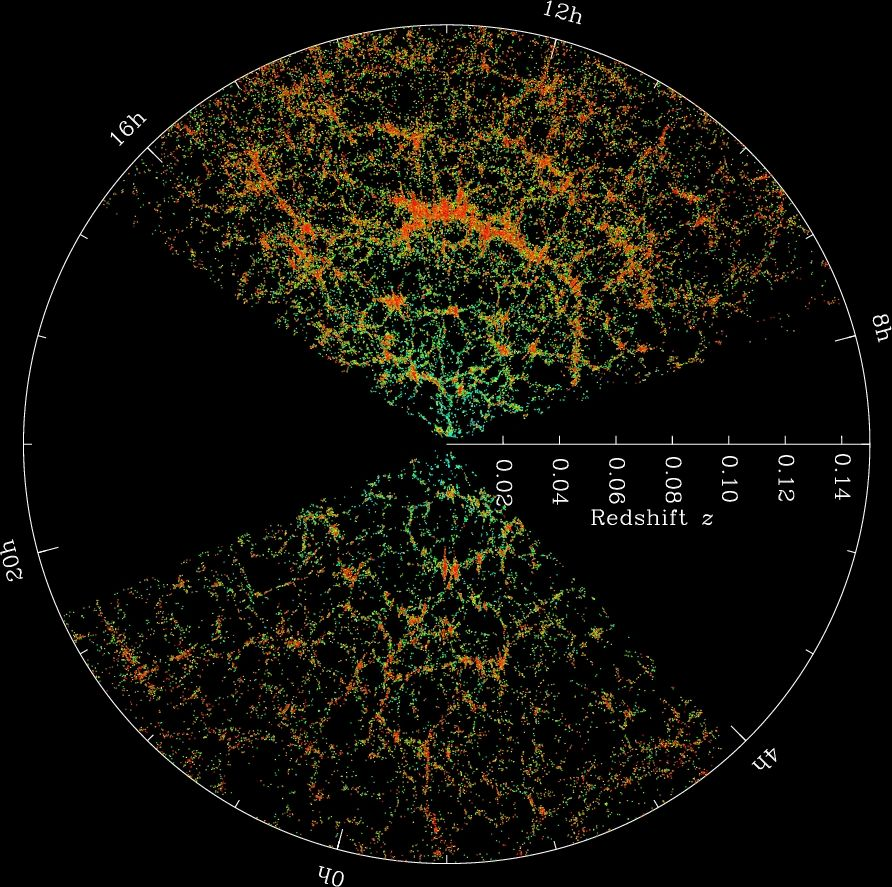
\includegraphics[width=0.9\linewidth]{orangepie}
	\caption{ Large Scale Structure (LSS) revealed by \cite{cite_sdss}}
	\label{fig:orangepie}
\end{figure}
\noindent
Understanding the statistical properties of the large scale structure and its evolution is crucial to test and constrain cosmological models. Computer simulations can be used to evolve initial inhomogeneities to the structure we see today and hence can compared with sky survey observations.


\section{Analytical tools}
Though the evolution of large scale structure can be simulated, we need analytical tools to get a deeper understanding and also to make generic constraints that can be tested by observations. On the other hand, simulations help in making and refining these analytical tools. A large fraction of the matter in the Universe is dark matter and it interacts only by gravity. Let us consider the standard $\Lambda$CMD model without any curvature.\\

\subsection{FLRW background}
The background FLRW metric in comoving coordinates is
\begin{align}
ds^2 &= -dt^2 + a^2(t) d\vec{x}^2\\
&= a^2(\tau) \left( -d\tau^2 + d\vec{x}^2 \right) 
\end{align}
where $\tau$ is defined as the conformal time.\\
Let $\bar{\rho}_{m}$ and $\bar{\rho}_{\Lambda}$ denote the mean matter density and mean dark energy density. Hubble parameter is defined as $H \equiv \dot{a}/a$ where the dot denotes derivative with respect to time '$t$'. At the zeroth order, the Einstein equations reduces to the Friedmann equations,
\begin{align}
%H^2 = \frac{8 \pi G}{3} \bar{\rho} = \frac{8 \pi G}{3} \left( \bar{\rho}_{m} + \bar{\rho}_{\Lambda} \right) \\ 
\nonumber
H^2 = \left(\frac{\dot{a}}{a}\right)^2 &= \frac{8 \pi G}{3} \bar{\rho} \\
\label{eq:fried-eqn-1}
&= \frac{8 \pi G}{3} \left( \bar{\rho}_{m} + \bar{\rho}_{\Lambda} \right) \\
\nonumber
\dot{H} + H^2 = \frac{\ddot{a}}{a} &= - \frac{4\pi G}{3} \left(\bar{\rho} + 3\bar{p} \right)\\
\nonumber
&= - \frac{4\pi G}{3} \left[ \bar{\rho}_{m} + \bar{\rho}_{\Lambda} + 3 (-\bar{\rho}_{\Lambda}) \right]\\
\label{eq:fried-eqn-2}
&= - \frac{4\pi G}{3} \left[ \bar{\rho}_{m} - 2 \bar{\rho}_{\Lambda} \right] 
\end{align}
%
Assuming that the matter and dark energy are independently conserved,
\begin{align}
\dot{\bar{\rho}}_{m} &= -3 H \left(\bar{\rho}_{m} + {\bar{p}_{m}}\right) = - 3 H \bar{\rho}_{m} \\
\dot{\bar{\rho}}_{\lambda} &= -3 H \left(\bar{\rho}_{\lambda} + \bar{p}_{\lambda} \right) = 0
\end{align}
Density parameter is defined as
\begin{align}
\Omega_{m} &\equiv \frac{8 \pi G \bar{\rho}_{m}}{3 H^2}\\
\Omega_{\lambda} &\equiv \frac{8 \pi G \bar{\rho}_{\lambda}}{3 H^2}
\end{align}
%
so that the first friedmann equation \ref{eq:fried-eqn-1} reduces to $\Omega_{m} + \Omega_{\lambda} = 1$. Let us now switch to conformal time '$\tau$' and define conformal Hubble parameter $\mathcal{H} \equiv \partial_\tau a / a = \dot{a}$. 


\subsection{Growth of Structure}
While the evolution of background cosmology can be studied fully analytically, the inhomogenities responsible for structure formation can't be solved exactly without making any ansatz. Let us define $\delta$ to indicate matter density contrast,
\begin{align}
\nonumber
\delta (\vec{x}, \tau) &\equiv \frac{{\rho}_{m} (\vec{x}, \tau) -\bar{\rho}_{m} (\tau) }{\bar{\rho}_{m} (\tau)} \\
&= \frac{{\rho}_{m} (\vec{x}, \tau) }{\bar{\rho}_{m} (\tau)} - 1
\end{align}
The velocity field is
\begin{align}
\vec{v} (\vec{x}, \tau) &= \frac{d \vec{r}}{dt} = \frac{d }{dt} (a \vec{x})\\
&= \frac{1}{a} \frac{d }{d \tau} (a \vec{x})\\
&= \frac{da/d \tau}{a} \vec{x} + \frac{d \vec{x}}{d \tau}\\
&= \mathcal{H} \vec{x} + \vec{u}
\end{align}
where $\vec{u}$ is defined as the peculiar velocity.

Evolution of $\delta, \vec{v}$ is described by the continuity equation, Euler equation and Poisson equation.
\begin{align}
\partial_{\tau} \delta + \nabla \cdot \left[ (1+ \delta) \vec{u} \right] &= 0\\
\partial_{\tau} \vec{u} + \mathcal{H} \vec{u} + \left( \vec{u} \cdot \nabla \right)  \vec{u} &= \nabla \Phi\\
\nabla^2 \Phi &= \frac{3}{2} \Omega_{m}(\tau) \mathcal{H}^2 \delta
\end{align}
where $\nabla$ is with respect to comoving coordinates and $\Phi$ is the gravitational potential





\subsubsection{Newtonian equations for inhomogeneous CDM}


\subsubsection{Linear solutions to inhomogeneous CDM}

\begin{align}
\end{align}

\subsubsection{Eulerian - 2nd order perturbation theory}

\subsubsection{Lagrangian approach - Zel'dovich approximations}

\subsubsection{Spherical collapse}

\subsection{Correlation function power spectrum relation}

\begin{align}
P(\vec{k}) &= \int \xi(\vec{r}) ~e^{i \vec{k} \dot \vec{r}} ~d^3r\\
\xi(\vec{r}) &= \frac{1}{(2\pi)^3} \int P(\vec{k}) ~e^{-i \vec{k} \dot \vec{r}} ~d^3 k\\
\xi(r) &= \frac{4 \pi}{(2\pi)^3} \int_{0}^{\infty} P(k) ~k^2 ~\frac{\sin(kr)}{kr} dk\\
\xi(r) &= \frac{1}{2\pi^2} \int_{-\infty}^{\infty} P(k) ~k^3 ~\frac{\sin(kr)}{kr} d(\ln k)\\
\xi(r) &= \int_{-\infty}^{\infty} \Delta^2(k) ~\frac{\sin(kr)}{kr} d(\ln k)
\end{align}

%\section{Background}
%Spherical collapse


\section{N-body simulations}

%\subsection{Particle approach}
%
%\subsection{Grid approach}


\section{Analysing a snapshot of a GADGET-2 simulation}
\cite{aseem_shadab}

\begin{figure}[H]
	\centering
	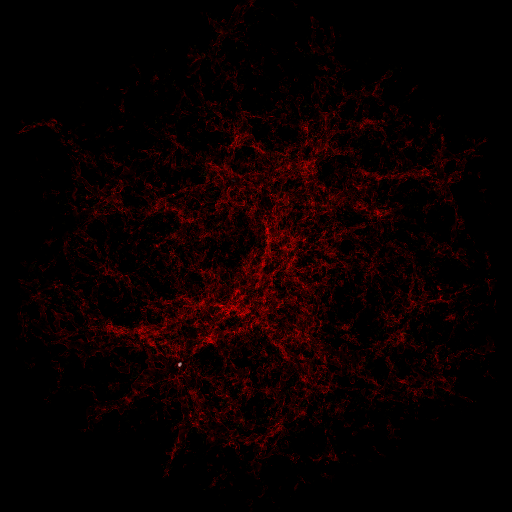
\includegraphics[width=0.9\linewidth]{../density_assign/UniformGridData_Render_density}
	\caption{Density field from the snapshot \quad
		 Volume rendered with yt-project}
	\label{fig:uniformgriddatarenderdensity}
\end{figure}


\section{Conclusion and Future plan}




\begin{thebibliography}{widest entry}
%\bibitem[GADGET]{cite_key1} bibliographic information
\bibitem[SDSS]{cite_sdss} \url{https://www.sdss.org/science/}
\bibitem[simulation]{aseem_shadab} Aseem Paranjape, Shadab Alam, Voronoi volume function: a new probe of cosmology and galaxy evolution, Monthly Notices of the Royal Astronomical Society, Volume 495, Issue 3, July 2020, Pages 3233–3251, \url{https://doi.org/10.1093/mnras/staa1379}
\end{thebibliography}






\end{document}